\chapter{Introduzione}
\section{Nozioni base}

L'obbiettivo di questo progetto \`e l'implementazione in \texttt{LifeV} di un risolutore ADR 3D, basato sulla tecnica di Riduzione Gerarchica di Modello (Hierarchical Model Reducation - HiMod). Consideriamo il seguente problema stazionario ai limiti:

\begin{equation}
\label{eq: problema forte}
\begin{cases}
-\mu\Delta u + \vect{b}\cdot \nabla u + \sigma u = f & \text{in $\Omega$}\\
u=u_{in} & \text{su $\Gamma_{in}$}\\
\frac{\partial u}{\partial \vect{n}}=0 & \text{su $\Gamma_{out}$ }\\
u=0 & \text{su $\Gamma _{vaso}$} \\
\end{cases}
\end{equation}


\begin{equation}
\label{eq:volume ridotto}
\Omega=\bigcup_{x\in \Omega_{1D}}\gamma_x
\end{equation}

\begin{center}
\begin{tikzpicture}
[scale=1.5]

\draw [thick] (2,0) rectangle (3,1);
\node at (-0.25,1.25) {$\Gamma_{in}$};
\node at (3.3,0.5) {$\Gamma_{out}$};
\node at (2,1.75) {$\Gamma_{vaso}$};
\node at (0.5,0.4) {$\gamma_{x}$};
%\node at (0.7,0.88) {$\gamma_{x}$};


\draw [thick] (2,1)--(0,2)--(1,2)--(3,1);
\draw [thick] (2,0)--(0,1)--(0,2);

\draw [dashed,thick] (0,1)--(1,1)--(1,2);
\draw [dashed,thick] (1,1)--(3,0);

\draw [pattern=north west lines, pattern color=gray, thick] (0.5,0.75) rectangle (1.5,1.75);

\draw [thick,dashed, ->] (-0.5,2)--(3.5,0);

\end{tikzpicture}
\end{center}

Immaginiamo di suddividere il dominio $\Omega$ in slice poste trasversalmente alla direzione longitudinale. Ognuna di queste slice verr\`a indicata con $\Omega_{1D}$.

Lungo $\gamma_x$ vengono utilizzate funzioni spaziali differenti rispetto a quelle utilizzate lungo $\Omega_{1D}$. Si consideri infatti per $\Omega_{1D}$, lo spazio funzionale $V_{1D}=H^1_{\Gamma_{in}}(\Omega_{1D})$, mentre sulla generica $\gamma_x$ si introducano le basi modali $\left\{ \varphi_k(y,z) \right\}$ ortonormali in $L^2(\gamma_x)$, con $k \in \mathbb{N}$.
Quest'ultime definiscono su $\gamma_x$ lo spazio funzionale $V_{\gamma_x}:=span\{\varphi_k\}$.

Definiamo ora il sottospazio generato solo dai primi m modi ovvero  $V^m_{\gamma_x}:=span\{\varphi_1,...,\varphi_m\}$ e combiniamolo con $V_{1D}$, il risultato di tale operazione \`e il seguente spazio ridotto:
\begin{equation}
\label{spazio: ridotto}
V_m:=\left\{v_m(x,y,z)=\sum^m_{k=1}\varphi_k(y,z)\tilde{v}_k(x) ,\:\:con\:\:\tilde{v}_k\in V_{1D}\right\}
\end{equation}

Questo \`e l'ambiente funzionale in cui opera il metodo HiMod.
L'ortogonalit\'a in $L^2(\gamma_x)$ implica che i coefficienti  $\tilde{v}_k$ in (\ref{spazio: ridotto}) sono il risultato del seguente prodotto scalare per $k=1,...,m$:
\begin{displaymath}
\tilde{v}_k(x)=\int_{\gamma_x}\varphi_k(y,z)v_m(x,y,z)\,dydz
\end{displaymath}
La convergenza di una soluzione $u_m$ tale che soddisfi il problema \eqref{eq: problema forte} \`e stata dimostrata (\textcolor{red}{citazione}). Valgono inoltre le seguenti propriet\`a:
\begin{itemize}
\item[-] $V_m \subset V$ $\forall m\in \mathbb{N}$, ossia che lo spazio ridotto $V_m$ \`e \textbf{conforme} in $V$;
\item[-] $\displaystyle \lim_{x\to +\infty} \left(\inf_{v_m\in V_m}\mid\mid v-v_m\mid\mid\right)=0$ 
per ogni $v \in V$, ossia che vale la \textbf{propriet\`a di approssimazione} di $V_m$ rispetto a $V$;
\end{itemize}
Le propriet\`a continuano a valere anche nel caso di dato di Dirichlet non omogeneo sulle pareti del vaso (\cite{perotto:2009}).

\section{Forma matriciale}

Per ogni $m\in\mathbb{N}$ consideriamo il seguente problema ridotto di \eqref{eq: problema forte}, 
trovare $u_m\in V_m$ tale che $\forall v_m\in V_m$:

\begin{multline}
\int_\Omega\left(\mu\nabla u_m\nabla v_m + \vect{b}\nabla u_mv_m+\sigma u_mv_m\right)\,d\Omega
=\int_\Omega fv \,dxdy
\end{multline}

Adoperiamo l'espansione tramite i coefficienti di Fourier della $u_m(x,y,z)=\sum_{j=k}^m\tilde{u}_j(x)\varphi _j(y,z)$ dove:
\begin{displaymath}
\tilde{u}_j(x)=\int_{\gamma(x)}u_m(x,y,z) \varphi_j(y,z)\,dydz
\end{displaymath}
consideriamo inoltre le funzioni test $v_m=\vartheta(x)\varphi _k(y,z)$ con $\vartheta(x)\in V_{1D}$ e $k=1,...m$. Il problema assume la seguente forma:

\begin{multline}
\sum_{j=1}^m \Bigg[
\int_\Omega\mu\nabla (\tilde{u}_j(x)\varphi _j(y,z))\nabla (\vartheta(x)\varphi _k(y,z))\,dxdydz\\
+\int_\Omega\vect{b}\nabla (\tilde{u}_j(x)\varphi _j(y,z)\vartheta(x)\varphi _k(y,z)\,dxdydz\\
+\int_\Omega\sigma\tilde{u}_j(x)\varphi _j(y,z)\vartheta(x)\varphi _k(y,z)\,dxdydz \Bigg] \\
=\int_\Omega f\vartheta(x)\varphi _k(y,z)\,dxdydz\\
\end{multline}

Svolgendo l'operatore gradiente si ottiene:

\begin{multline}
\sum_{j=1}^m \Bigg[
\int_\Omega\mu( \partial_x\tilde{u}_j \partial_x\vartheta\varphi _j\varphi _k + \tilde{u}_j \vartheta \partial_y\varphi _j\partial_y\varphi _k + \tilde{u}_j \vartheta \partial_z\varphi _j\partial_z\varphi _k)\,dxdydz \\
+ \int_\Omega (b_1\partial_x\tilde{u}_j\varphi _j+b_2\tilde{u}_j\partial_y\varphi _j + b_3\tilde{u}_j\partial_z\varphi_j)\vartheta\varphi _k\,dxdydz\\ 
+ \int_\Omega \sigma\tilde{u}_j\vartheta\varphi _j\varphi _k\,dxdydz \Bigg]\\
=\int_\Omega f\vartheta\varphi _k\,dxdydz
\end{multline}


Definiamo con N il numero di nodi scelti, uniformemente distribuiti lungo $\Omega_{1D}$. La partizione $T_h$, costruita lungo la fibra di supporto 1D, avr\`a un passo spaziale $h=\vert \Omega_{1D}\vert / (N-1)$. Introduciamo lo spazio agli elementi finiti lungo $\Omega_{1D}$ definito come segue

\begin{equation}
\label{eq: spazio polinomiale}
X_h^r= \left\{\psi_h \in C^0(\Omega_{1D}): \psi_h \vert_K  \in \mathbb{P}_r,\forall K\in T_h \right\}\footnotemark
\end{equation}

\footnotetext{Il codice \`e stato scritto in modo da utilizzare polinomi di primo grado, la generalizzazione non rientrava negli obbiettivi primali del progetto}

Possiamo quindi esprimere i coefficienti di Fuorier nel seguente modo: 
\begin{equation}
\label{eq: coeff fourier espansi}
\tilde{u}_j(x)=\sum_{s=1}^Nu_{js}\psi_s(x)
\end{equation}

 
 Otteniamo la formulazione matriciale del nostro problema ovvero, trovare $\vect{u} \in \mathbb{R}^{N*m}$ tale che $\forall \psi_l$ e $\forall \varphi_k$, con $l=1,...N$ e $k=1,...m$ si ha che:

\begin{multline}
\sum_{j=1}^m \sum_{s=1}^N
u_{js} \Bigg[ \int_\Omega\mu( \partial_x\psi_s \partial_x\psi_l\varphi _j\varphi _k + \psi_s \psi_l \partial_y\varphi _j\partial_y\varphi _k + \psi_s \psi_l \partial_z\varphi _j\partial_z\varphi _k)\,dxdydz \\
+ \int_\Omega (b_1\partial_x\psi_s\varphi _j+b_2\psi_s\partial_y\varphi _j + b_3\psi_s\partial_z\varphi_j)\psi_l\varphi _k\,dxdydz\\ 
+\int_\Omega \sigma\psi_s\psi_l\varphi _j\varphi _k\,dxdydz \Bigg]\\
=\int_\Omega f\psi_l\varphi _k\,dxdydz
\end{multline}

 Osserviamo che il doppio indice $"js"$, in realt\`a scorre un vettore, la rimappatura in un solo indice pu\`o 
 facilmente essere dedotta ottenenedo che $[\vect{u}]_{js}=\vect{u}[(j-1)N+s]$. 
 
 La matrice generata ha dimensioni $(mN)^2$, tuttavia fissata la frequenza delle soluzione e della funzione test \`e 
 possibile identificare un blocco che corrisponde ad un problema monodimensionale.
 Se utilizziamo, in direzione x, gli elementi finiti di grado 1, il blocco risulta tridiagonale e, in questo caso, la matrice ha un numero di elementi non zero pari a $m^2(3N-2)$. Il pattern\footnotemark di sparsit\`a per un caso con m=3 e N=14 \`e riportato in figura \ref{fig:pattern}.
 
 \begin{figure}[h]
    \centering
    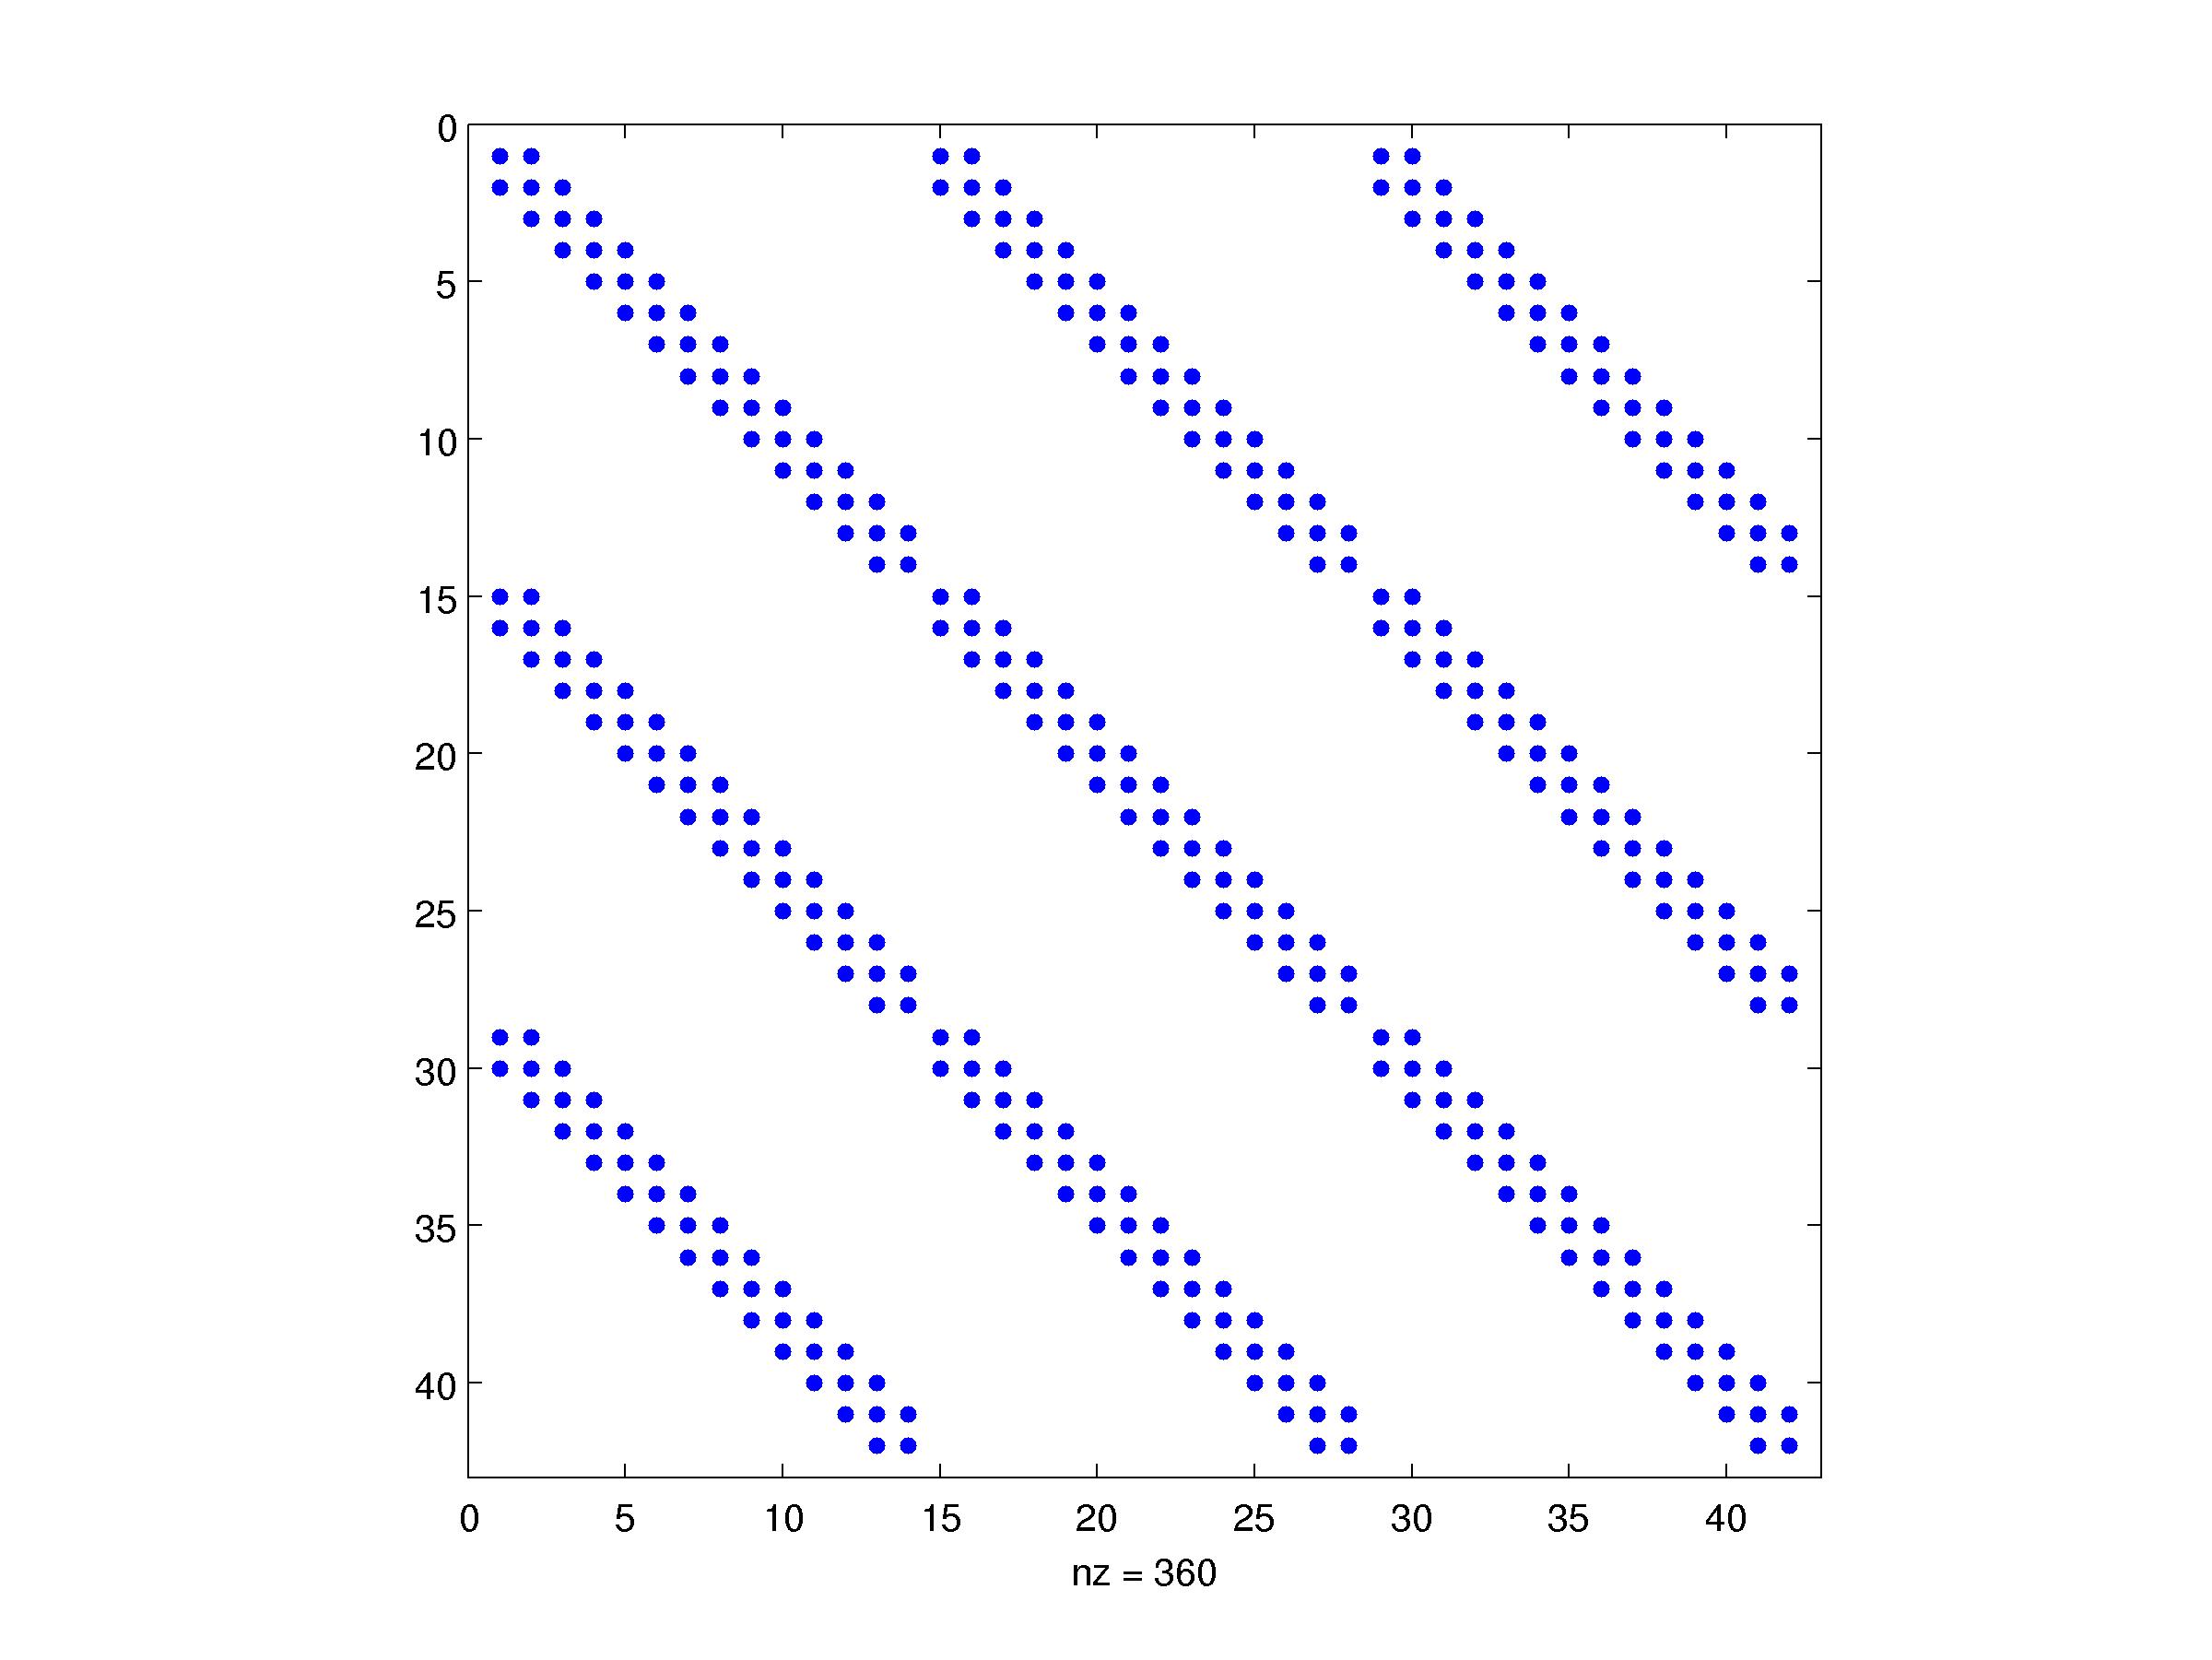
\includegraphics[scale = 0.45]{spy_14elem3modes}
    \caption{Pattern di sparsit\`a per un caso con 14 elementi P1 e 3 modi.}
    \label{fig:pattern}
\end{figure}

\footnotetext{La matrice dei coefficienti \`e dunque sparsa ed inoltre il pattern \`e noto a priori, queste 
 informazioni hanno permesso un assemblaggio pi\`u veloce in sede implementativa. 
}

\section{Educated Basis}\label{sec: educated basis}
\

Introduciamo con degli esempi l'algoritmo di ricerca delle basi ortonormali, senza entrare nel dettaglio della teoria;

\begin{itemize}
\item[\textbf{1.}] \textbf{Costruzione di un problema ausiliario} che rispecchi la natura delle condizioni alle pareti del problema originale (devono essere omogenee) e passaggio ai relativi problemi agli autovalori.
\mybox{
Nel caso si abbiano condizioni di robin uguali sull'intera parete del vaso, dovremo considerare il seguente problema ausiliario:
\begin{equation}
\label{eq: problema RRRR}
\begin{cases}
-\Delta u(y,z)= 0 & \text{in $\gamma_x$}\\
\mu \nabla u(y,z) \cdot \vect{n}_{\gamma_x} +\chi u(y,z)=0 & \text{su $\Gamma_{vaso}$} \\
\end{cases}
\end{equation}
Si passi ora al problema agli autovalori associato al precedente sistema e ipotizzando la separazione di variabili per $u(y,z)=\varphi(y)\vartheta(z)$, si arrivano facilmente ad ottenere i seguenti sottoproblemi agli autovalori:
\begin{equation}
\label{eq: problema RR1}
\begin{cases}
-\varphi(y)'' = K_y\varphi(y) & \\
\mu \varphi(y)' +\chi \varphi(y) = 0 & \text{per $y=L_y$} \\
-\mu \varphi(y)'+\chi \varphi(y)=0 & \text{per $y=0$} \\
\end{cases}
\end{equation}
\begin{equation}
\label{eq: problema RR2}
\begin{cases}
-\vartheta(z)'' = K_z\vartheta(z) & \\
\mu \vartheta(z)' +\chi \vartheta(z) = 0 & \text{per $z=L_z$} \\
-\mu \vartheta(z)'+\chi \vartheta(z)=0 & \text{per $z=0$} \\
\end{cases}
\end{equation}
}{Esempio - RRRR}

\item[\textbf{2.}] \textbf{Identificazione del tipo di soluzione} dei problemi agli autovalori associati.

\mybox{
Per i sottoproblemi ottenuti i generi di soluzione sono i seguenti:
\begin{equation}
\label{eq: 1sottoproblema}
\begin{array}{c}
\varphi (y)=Asin(\sqrt{K_y}y)+Bcos(\sqrt{K_y}y) \\ \\
\vartheta (z)=Asin(\sqrt{K_z}z)+Bcos(\sqrt{K_z}z)
\end{array}
\end{equation}

}{Esempio - RRRR}

\item[\textbf{3.}] \textbf{Ricerca degli autovalori di un sottoproblema} tramite risoluzione dell'equazione non lineare associata ad esso, ottenuta risolvendo le condizioni di bordo.
\mybox{
Nel caso trattato in esempio le equazioni che si ottengono sono le seguenti ($x = \sqrt{K_y}$ e $w= \sqrt{K_z}$):
\begin{equation}
\label{eq: funzione autovalori}
\begin{array}{c}
f(x)= 2\mu x + tan(L_y x)\left(\chi - \frac{\mu ^2 x^2 }{\chi} \right) \\ \\
f(w)= 2\mu w + tan(L_z w)\left(\chi - \frac{\mu ^2 w^2 }{\chi} \right)
\end{array}
\end{equation}
}{Esempio - RRRR}
\end{itemize}

\mybox{
Nel caso di condizioni al bordo di Dirichlet il problema si semplifica. Infatti non occorre adottare l'algoritmo mostrato precedentemente, gli autovalori che si ottengono sono noti a priori e sono della forma:
\begin{equation}
\label{eq: problema agli autovalori dirichlet}
\begin{array}{c l}
K_y = \big( \frac{\pi p}{L_y}\big)^2 & p = 1, ... ,m_y\\
K_z = \big( \frac{\pi q}{L_z}\big)^2 & q = 1, ... ,m_z\\
\end{array}
\end{equation}
Dunque \'e nota la relazione $\lambda(K_y,K_z)$ a priori e risulta molto semplice ordinare in modo crescente gli autovalori definendo quindi $m_y$ e $m_z$.
}{Osservazione}

\section{Ipotesi}\label{sec: ipotesi}

Le ipotesi alla base di questo progetto sono le seguenti:

\begin{itemize}
\item Il dominio di calcolo \`e un parallelepipedo che si estende nell'ottante positivo.
\item I coefficienti della forma sono assunti costanti.
\item Viene risolto un problema ADR stazionario con condizioni di inflow di tipo Dirichlet e di outflow di tipo Neumann omogeneo.
\item Condizioni sulle pareti omogenee.
\item \`E possibile separare il problema lungo le direzioni trasversali, in due sotto problemi agli autovalori.
\end{itemize}

La forma del dominio considerato ci consente agilmente di applicare le tecninche di separazione di variabili e utilizzare la teoria delle basi educate. Pi\`u delicata risulterebbe la gestione di condizioni di bordo sulla parete del vaso, nel caso di sezione a forma generica. Nei capitoli successivi verranno accennate le difficolt\`a che presenta questa tematica.
Anche nel caso di generalizzazione dei coefficienti della forma, viene presentata una soluzione possibile, tuttavia il codice \`e strutturato per l'utilizzo di coefficienti costanti. In ogni caso consideriamo termini forzanti non costanti lungo il dominio.
Per quanto il problema a sezione cilindrica potesse sembrare uno stretto parente del parallelepipedo cos\`i non \`e; renderemo chiare le principali differenze, insite nell'equazione risultante dalla separazione di variabili.
Per quanto riguarda le condizioni di inflow, il codice permette di applicare condizioni di Dirichlet non omogenee, tale generalit\`a non vale per la condizione di Neuamann all'outflow, ma l'eventuale estensione \`e triviale, dato che \`e sufficiente modificare opportunamente la forma bilineare.

Dalla teoria di HiMod sar\`a ormai chiaro che nella discretizzazione del dominio si fondono due concezioni molto diverse, da una parte gli Elementi Finiti lungo la fibra di supporto, dall'altra la base modale 2D, che ricorda molto i metodi spettrali. 
Dunque l'organizzazione delle classi \`e seguita naturalmente dalle necessit\`del metodo. Avevamo bisogno inizialmente di una classe che ci permettesse di maneggiare gli elementi dello spazio modale, ovvero la classe \textbf{ModalSpace}, ottenuto questo primo risultato \`e stata creata la classe che mette in comunicazione la fibra di supporto con le slices e risolve il problema, ovvero \textbf{HiModAssembler}. Il terzo soggetto principale di questo lavoro \`e \textbf{Basis1DAbstract}, ovvero la classe su cui si appoggia ModalSpace per costruire le basi modali basate sulla teoria delle basi educate.
Nel prossimo capitolo analizzeremo nel dettaglio queste tre colonne portanti del codice.